
\chapter{Química Cuantitativa}

\section{Introducción}
Se define la Química (del egipcio \emph{Keme}, “tierra”) como la ciencia que estudia la estructura, propiedades, composición y transformación de la materia. La química moderna se desarrolló a partir de la alquimia, una práctica protocientífica de carácter filosófico, que combinaba elementos de la química, la metalurgia, la física, la medicina, la biología, entre otras ciencias y artes. Esta fase termina al ocurrir la llamada,Revolución de la Química, basada en la Ley de conservación de la Masa y la teoría de la combustión por oxígeno postuladas por el científico francés, Antoine L. Lavoisier. \\
La Química a veces es definida como La Ciencia Central a causa de su rol de conexión y articulación entre las ciencias físicas, de las cuales forma parte, junto con las ciencias de la vida, y algunas ciencias aplicadas como la medicina o la ingeniería.

\section{Leyes Ponerales}

Las leyes ponderales de la Química son un conjunto de leyes de carácter empírico desarrolladas entre 1789 y 1803 por los primeros químicos que trataban de encontrar relaciones entre las masas de los compuestos químicos que intervenían en una reacción química. Posteriormente fueron generalizadas y superadas con la aparición de la teoría atómica y el concepto de mol.

\subsection{Ley de la Conservación de la Masa (Ley de Lavoisier)}

\textbf{Antonie-Laurent de Lavoisier (1743-1794)}, fue el primer químico que realizó cuidadosamente mediciones con la balanza, obteniendo una explicación correcta de las reacciones en las que metales como mercurio o cobre eran calentados en presencia de aire. En 1789, Lavoisier generalizó sus resultados a todas las reacciones químicas enunciando la llamada \emph{Ley de conservación de la masa}:\\

\begin{law}[Ley de Lavoisier]
En una reacción química, la masa total de las substancias que reaccionan (reactivos) es igual a la masa total de las substancias formadas (productos)
\begin{align}
\sum_{i = 1}^{N}(m_i)_{reactivos} = \sum_{i = 1}^{N}(m_i)_{productos}
\end{align}
\end{law}
\begin{figure}[h!]
	\centering
	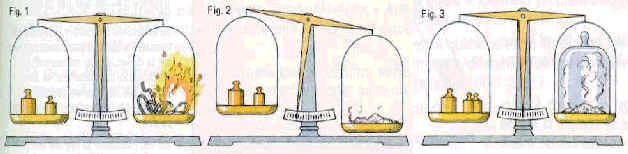
\includegraphics[width=0.8\textwidth]{lavoisier}
	\caption{Representación gráfica de las experiencias de Lavoisier}
\end{figure}

\subsection{Ley de las Proporciones Definidas (Ley de Proust)}

Si en condiciones cuidadosamente controladas, hacemos reaccionar por ejemplo, 10 g de cloro con 10 g de sodio, podrá probarse que los 10 g de cloro no reaccionan con todo el sodio, sino solo con una porción de él (6,484 g exactamente) quedándose el exceso sin reaccionar. Según la experiencia, el cloro y el sodio han reaccionado en la proporción en peso:\\

\begin{center}
	$\frac{m_{Na}}{m_{Cl}}=\frac{6,484}{10}$
\end{center}

\begin{law}[Ley de Proust]
	Cuando dos o más elementos se combinan para formar un determinado compuesto lo hacen en una relación en peso constante independientemente del proceso seguido para formarlo.
\end{law}

Esta ley fue enunciada por \emph{Louis Proust} en 1799, y atacada por \emph{C. L. Berthollet}, quién creía que la composición de un compuesto variaba según el método por el que se había preparado.\\

Modernamente se conocen compuestos sólidos que no cumplen la ley de las proporciones definidas (óxidos y sulfuras de elementos de transición), y se les llama compuestos no estequiométricos o \emph{Compuestos Berthóllidos}.\\

Podemos decir por tanto que:

\begin{center}
		$\frac{m_{Na}}{m_{Cl}}=\frac{6,484}{10}=\frac{12,968}{20}=\frac{4,934}{7,61}=cte$
\end{center}

Cada muestra de sal común descompuesta nos arrojará invariablemente un 39,34 \% de sodio y un 60,66 \% de cloro (relación 6,484/10)

\subsection{Ley de las Proporciones Múltiples (Ley de Dalton)}

La ley anterior no excluye la posibilidad de que dos sustancias puedan formar compuestos diferentes si varían las condiciones experimentales. De hecho, esto es lo que sucede, por ejemplo, con el oxígeno y el hierro o el cobre o el carbono, que dependiendo de las condiciones de la experiencia se originan óxidos diferentes. Para cada proceso individual, se cumple, por supuesto la ley de Proust, sin embargo, cabe hablar de otra más general que incluye estos casos. Veamos un ejemplo:\\

Al hacer reaccionar un gramo de oxígeno con cobre, la cantidad de éste consumida es exactamente 3,971 g:

\begin{center}
	$Oxígeno (1 gr) + Cobre  (3,971 gr) \rightarrow Óxido de Cobre
	$ 
\end{center}

Pero en condiciones experimentales diferentes, un gramo de oxígeno puede reaccionar con 7,942 g de cobre para dar lugar a otro compuesto diferente:

\begin{center}
	$Oxígeno (1 gr) + Cobre (7,942 gr) \rightarrow Óxido de Cobre’ $
\end{center}

Si dividimos los gramos de cobre que en ambos casos se combinaron con la misma cantidad (un gramo) de oxígeno, veremos que resulta una relación muy sencilla:

\begin{center}
	$\frac{3,971}{7,942}=\frac{1}{2}$
\end{center}

Lo anterior es un ejemplo de la Ley de las Proporciones Múltiples enunciada en 1803 por \emph{J. Dalton}:\\

\begin{law}[Ley de Dalton de las Proporciones Múltiple]
	Las cantidades de un mismo elemento que se combinan con una cantidad fija de otro para formar varios compuestos están en la relación de los números enteros sencillos
\end{law}

\subsection{Ley de las Proporciones Equivalentes (Ley de Richter)}

Fue enunciada por primera vez por \emph{J.B. Richter} en 1792. Es de importancia para la historia de la química y el desarrollo del concepto de mol y de fórmula química más que para la química actual. Esta ley permite establecer el peso equivalente o peso-equivalente-gramo, que es la cantidad de un elemento o compuesto que reaccionará con una cantidad fija de una sustancia de referencia.\\

\begin{law}[Ley de Richter]
	
	Las masas de dos elementos diferentes que se combinan con una misma cantidad de un tercer elemento, guardan la misma relación que las masas de aquellos elementos cuando se combinan entre sí.
\end{law}

\section{Teoría Atómica de Dalton}

El Químico inglés \emph{John Dalton (1766-1844)} fue uno de los primeros que reflexionó sobre estas leyes empíricas y otras leyes sobre el comportamiento de los gases, llegando a la conclusión de que los elementos químicos deberían estar constituidos por partículas pequeñísimas e indivisibles a las que denominó átomos. Mucho tiempo antes que él, el griego \emph{Demócrito de Abdera} había propuesto esta misma denominación para explicar los constituyentes íntimos de la materia. Dalton adoptó el mismo término. La llamada \textbf{Teoría Atómica de Dalton} establecía como puntos fundamentales que:

\begin{itemize}
	\item Los elementos químicos están formados por partículas (átomos) que son indivisibles e inalterables en todo proceso químico.\\
	\item Todos los átomos de un mismo elemento son exactamente ¡guales entre sí y distintos a los átomos de otro elemento diferente.\\
	\item Los compuestos se originan por la unión intensa de átomos distintos en una proporción constante.
\end{itemize}

Con estas ideas, Dalton podía explicar las leyes ponderales conocidas. En efecto, si los átomos son inalterables y una reacción química no es más que la reordenación de átomos, deberá haber el mismo número de estos átomos en todo el proceso, por lo que la masa debería permanecer inalterada.

\section{Leyes Volumétricas}

Son un conjunto de leyes de naturaleza empírica que relaciona los volúmenes de gases que intervienen en una reacción química.

\subsection{Ley de los Volúmenes de Combinación de Gay-Lussac}

El químico francés \emph{Joseph Louis Gay-Lussac} (1778-1850) estudió las reacciones en las que intervenían gases, realizando sus estudios en reacciones a Presión y Temperatura constantes. Tras estudiar distintos tipos de reacciones químicas (siempre en fase gaseosa) llegó a la conclusión que ocurría algo análogo a la la Ley de Proust cuando se medían los distintos volúmenes de las sustancias intervinientes en la reacción.\\



\begin{law}[Ley de los Volúmenes de Combinación de Gay-Lussac]
	Los volúmenes de las sustancias gaseosas que intervienen en una reacción química, medidos en las mismas condiciones de presión y temperatura, están en relación de números enteros sencillos.
\end{law}

\begin{center}
	\textbf{Cuando Dalton recibió esta información encontró algo que no cuadraba con su teoría de átomos indivisibles.}\\
\end{center}

Si la reacción de formación de agua se da en esas proporciones es evidente que la fórmula del agua no es $HO$, sino $H_2O$. Esto fue aceptado por Dalton (es una manera de determinar fórmulas) y supuso la corrección de la escala de masas atómicas relativas: el átomo de oxígeno tiene una masa igual a la de 16 átomos de hidrógeno.\\

Dalton aceptó que dos átomos de hidrógeno se combinaban con un átomo de oxígeno. Pero esta combinación debía producir una partícula (él la llamó átomo- compuesto) de agua, y por tanto, el volumen de agua obtenido debía ser un litro. Como Gay-Lussac informó de la obtención de dos litros de vapor de agua, Dalton supuso que tales medidas no podían ser correctas. Sin embargo, los datos obtenidos en el laboratorio eran claros: Gay-Lussac no estaba equivocado, un litro de oxígeno se combina con dos litros de hidrógeno y produce dos litros de vapor de agua. La solución vendría de otro químico genial: \textbf{Amadeo Avogadro}.

\subsection{Hipótesis de Avogadro}

En sus hipótesis Avogadro sugiere que las partículas de los gases son en realidad de dimensiones mucho menores que el volumen del recipiente que las contienen, de forma que estas no están en reposo como creía Dalton, sino están muy separadas en continuo movimiento. Sin esta condición no parecería lógico que moléculas grandes o pequeñas ocuparan el mismo volumen. Pronto se comprobó que las partículas de los gases elementales son moléculas diatómicas y la primera utilidad fue la determinación de fórmulas de compuestos y, por tanto, la determinación de las masas atómicas relativas correctas.\\

Según Avogadro:

\begin{itemize}
	\item Cada molécula de agua debe tener, como mínimo, un átomo de oxígeno. Si el volumen de agua que se obtiene es el doble que el de oxígeno, la molécula de oxígeno debe ser diatómica, para que cada molécula origine los átomos que permitan formar dos moléculas de agua.\\
	\item Como el volumen de agua es el mismo que el de hidrógeno, debe haber el mismo número de moléculas de cada uno.
\end{itemize}

\begin{law}[Hipótesis de Avogadro]
	En condiciones iguales de presión y temperatura, volúmenes iguales de gases diferentes tienen el mismo número de moléculas....
\end{law}

\section{Concepto de Mol}

Determinar la masa de un átomo o de una molécula es evidentemente imposible usando las balanzas, de ahí que los químicos hayan decidido definir una "nueva" unidad para medir la masa de átomos y moléculas. A esa unidad se la denomina unidad de masa atómica (uma) y ya que el hidrógeno se ha comprobado que es el elemento de menos masa es lógico definirlo como unidad, definirlo como uma.\\

Así en una primera aproximación diremos que la unidad de masa atómica es simplemente la masa de un átomo de hidrógeno. De modo que si decimos que, por ejemplo, el carbono tiene de masa atómica 12 urna, con ello estamos diciendo que un átomo de carbono pesa 12 veces más que un átomo de hidrógeno, o si decimos que la molécula de agua pesa 18 urna, decimos que una molécula de agua pesa 18 veces más que un átomo de hidrógeno, y así sucesivamente.\\

Lógicamente la masa de una molécula (masa molecular) se obtendrá por la suma de las masas atómicas de cada uno de los elementos que la forman. Esos datos de masas atómicas vienen recogidas en la tabla periódica. Con todo, en los laboratorios las balanzas no miden uma, sino gramos, de ahí que haga falta hallar una relación entre ambas escalas.\\


Mil moléculas (o átomos) de cualquier especie es aún un número muy pequeño para poder pesarse en la balanza, pero todo es cuestión de escoger un número muy grande de moléculas (o átomos) que podamos pesar. Lógicamente, 1000 átomos de carbono, por ejemplo, pesarían en uma $12\cdot 1000$. Si en lugar de elegir mil elegimos $10^{23}$ resulta que ese es un número ya muy muy grande. Si escogemos $6,02\cdot10^{23}$ átomos de carbono, éstos pesarán $12\cdot6,02\cdot10^23$ uma, pero curiosamente, al poner todos esos átomos sobre la balanza, "curiosamente" pesan 12 gramos.\\

\begin{definition}[Mol]
	El mol corresponde con la cantidad de materia que contiene $6.022\cdot10^{23}$ átomos o moléculas de una determinada sustancia
\end{definition}

Esa es la ventaja de elegir “ese número tan raro", que \textbf{la masa en gramos de la especie elegida coincide numéricamente con la masa en uma}. A ese “número tan raro” se le conoce con el nombre de \textbf{Número de Avogadro}:\\

\begin{center}
$N_A=6,02\cdot10^{23}$
\end{center}
Por todo lo anteriormente expuesto aquí, existe una manera de calcular la equivalencia entre gramos y moles de una substancia:

\begin{definition}[Definición de Mol]
	Se define el Mol como los gramos de una determinada sustancia dividida por su masa molecular:
	\begin{align}
		& n=\frac{gr}{M_m}
	\end{align}
\end{definition}

\begin{exercise}
	\textbf{Calcula los moles de moléculas de Ácido Sulfúrico contenidas en 100 gr de dicha substancia. Calcula también los moles y el número de átomos de oxígeno.}\\
	
	La masa molecular del ácido sulfúrico ($H_2SO_4$) es:
	$M_m = 2\cdot1 + 1\cdot32 + 4\cdot16 = 98 gr/mol$\\
	
	El número de moles de Ácido Sulfúrico por tanto, es:
	$n = \frac{100}{98} = $1,021 moles de $H_2SO_4$\\
	
	Y el número de moléculas: 
	$1,021\cdot6,02\cdot10^{23} = 6,14\cdot10^{23}$  moléculas de $H_2SO_4$\\
	
	Puesto que existen 4 átomos de oxígeno por molécula de ácido sulfúrico:\\
	
	1,021 moles de $H_2SO_4 \cdot 4 = 4,84$ moles de átomos de oxígeno
	
	$4 \cdot 6,14 \cdot10^{23}$  moléculas de $H_2SO_4 = 2,46 \cdot10^{24}$ átomos de oxígeno
	
\end{exercise}

\section{Concepto de Equivalente}

Se define \emph{Equivalente o Equivalente Gramo} a la masa de una substancia dada que:\\

\begin{itemize}
	\item Sustituye o reacciona con un mol de iones hidrógeno ($H^+$) en una reacción ácido-base.\\
	\item Sustituye o reacciona con un mol de electrones en una reacción redox.\\
\end{itemize}

El concepto de equivalente es de gran utilidad sobre todo en reacciones ácido-base y redox, puesto que en dichas reacciones las sustancias intervinientes lo hacen equivalente a equivalente, lo cual simplifica muchísimo los cálculos. Se puede calcular:\\

\begin{definition}[Equivalente]
	
	Se define Equivalente como los gramos de cierta sustancia divididos entre su Masa Equivalente
	
	\begin{align}
		& eq =\frac{gr}{M_{eq}}
	\end{align}
	
\end{definition}

Como podemos observar la similitud con la definición de Mol es evidente, como evidente es también la semejanza entre Masa Equivalente y masa Masa Molecular:\\

\begin{definition}[Masa Equivalente]

Se define Masa Equivalente de una sustancia en una reacción química dada como la Masa Molecular de dicha sustancia entre su valencia en dicha reacción química, entendiendo por valencia el número de Hidrógenos intercambiados en una reacción ácido-base o el número de electrones cedidos o absorbidos en una reacción Redox

\begin{align}
	& M_{eq} = \frac{M_{m}}{Val}
\end{align}

\end{definition}

\section{Modelo del Gas Ideal}

Un gas ideal es un modelo teórico que explica el comportamiento de los gases, simplificando su comportamiento y permitiendo su estudio teórico de manera sencilla. Dicho modelo se basa en las siguientes premisas:
\\

\begin{enumerate}
	\item El número de partículas constituyentes del gas es muy grande, como también lo son las distancias entre ellas en comparación con el recipiente que las contiene. Por tanto, podemos considerar las partículas como masas puntuales con un volumen despreciable\\
	\item Las partículas que forman el gas se encuentran en continuo movimiento, caótico y muy rápido.\\
	\item Las partículas chocan entre si elásticamente. También se producen choques elásticos con las paredes del recipiente, siendo la Presión del gas el resultado macroscópico de dicho movimiento.\\
	\item Se consideran despreciables las fuerzas entre partículas, salvo en el momento de los choques. Esto implica que los gases ideales no licúan.\\
	\item El gas es considerado puro, es decir, todas las moléculas son iguales.\\
\end{enumerate}

Solo los gases mas ligeros en condiciones de bajas presiones y temperaturas tienen un comportamiento que se aproxima al del gas ideal. Sin embargo, las conclusiones extraídas de dicho modelo resultan altamente valiosas a la hora de estudiar (y entender) el comportamiento de los gases reales.

\subsection{Ecuación de Estado de los Gases Ideales}

Se definen las \emph{Variables de Estado} de un sistema como aquellas que por si mismas son capaces de definir totalmente el estado de un sistema fisicoquímico. En el caso de los gases, estas variables de estado son tres, a saber, \textbf{Presión, Volumen y Temperatura}.\\

Para el caso de los Gases Ideales, existe una ecuación que relaciona de manera extremadamente sencilla y eficaz las tres variables de estado. A esta relación se le conoce como \textbf{Ecuación de Estado de los Gases Ideales}:

\begin{definition}[Ecuación de Estado de los gases Ideales]
	El producto de la Presión a la que está sometido un Gas Ideal por su Volumen es directamente proporcional a la temperatura de éste:
	
	\begin{align}
		& P\cdot V = n\cdot R \cdot T
	\end{align}
	
\end{definition}

Donde P se mide en atmósferas, V en litros, n en moles y T en Kelvin. A R se le conoce como constante de los gases ideales, y su valor es $R = 0,082 atm \cdot l/ mol\cdot K$. La Ley de los gases ideales es totalmente coherente con las leyes de Gay-Lussac y Boyle-Mariotte estudiadas en cursos anteriores.\\

Una de las características mas destacables de la Ecuación de los Gases Ideales es que es totalmente independiente de de la naturaleza del gas que estemos estudiando, lo cual hace de ella una herramienta prácticamente universal.\\

\begin{exercise}
	\textbf{Calcula el Volumen que ocupará un mol de Gas Ideal medido en Condiciones Normales.}\\
	
	En Química se definen las Condiciones Normales (C.N) a aquellas correspondientes a P = 1 atm y T = 273 K. Por tanto:\\
	
	$V = \frac{n \cdot R \cdot T}{V} = \frac{1 \cdot 0,082 \cdot 273}{1} = 22,4 l$
		
\end{exercise}

Según lo dicho anteriormente, la ecuación de los gases ideales no depende de la naturaleza del gas. Por tanto se puede concluir que:\\

\begin{definition}[Volumen de un Gas Ideal en CN]
	Un mol de cualquier gas ideal medido en Condiciones Normales ocupa un Volumen de 22,4 l
\end{definition}

\subsection{Mezcla de Gases: Ley de Dalton de las Presiones Parciales}

Puesto que es casi imposible encontrar reactivos que sean químicamente puros, por norma general los gases se encuentran formando mezclas, por lo que su estudio se hace mas difícil. Fue el científico ingles J. Dalton quien en 1801 resolvió el problema enunciando la \textbf{Ley de las Presiones Parciales}\\

\begin{definition}[Presión Parcial de un gas]
	Se define la Presión Parcial de un gas en una mezcla como aquella que tendría dicho gas si en el recipiente que contiene la mezcla estuviese el solo a las mismas condiciones de Temperatura 
\end{definition}

Por tanto podemos enunciar:

\begin{law}[Ley de Dalton de las Presiones Parciales]
	La presión de una mezcla de gases ideales que no reaccionan químicamente, es igual a la suma de las presiones parciales que ejercería cada uno de ellos si sólo uno ocupase todo el volumen de la mezcla:\\
	
		$P_T = \displaystyle\sum_{i=1}^{N}P_i$\\
		
		$P_i = X_i \cdot P_T$
		
\end{law}

Donde $P_T$ es la presión total, $P_i$ la presión parcial de gas en la mezcla y $X_i$ la fracción molar del gas en dicha mezcla.\\

Si estamos ante el caso de un gas ideal, la ecuación de estado también se puede aplicar a cada gas por separado:

\begin{center}
	$P_i = n_i \cdot R \cdot T$
\end{center}

\section{Análisis Elemental y Composición Centesimal}

Uno de los primeros problemas al que se enfrenta un químico cuando se encuentra ante un compuesto químico desconocido es hallar cual es su composición. Esto es de vital de importancia si nos encontramos ante un compuesto orgánico, en donde el primer paso será siempre el encontrar su formula molecular, como actuación previa para poder determinar su estructura. Así definimos composición centesimal como el porcentaje en masa de cada uno de los elementos que forman un compuesto en relación a la masa total.

\begin{exercise}
	\textbf{Indica la Fórmula Molecular de un compuesto químico que contiene 40 \% de C, 6,7 \% de H y 53,3 \% de O. Su masa molecular obtenida por espectrometría de masas es 60 gr/mol.}\\
	
	Dividimos cada uno de los porcentajes entre su masa atómica:\\
	
	$C: \frac{40}{12}=3,33$
	$H: \frac{6,7}{1}=6,7$ 
	$O: \frac{53,3}{16}=3,33$\\
	
	A continuación dividimos entre el número más bajo para establecer la proporción:\\
	
	$C: \frac{3,33}{3,33}=1$
	$H: \frac{6,7}{3,33} \simeq 2$ 
	$O: \frac{53,3}{16}=1$\\
	
	Por tanto la fórmula empírica del compuesto es $(CH_2O)_x$, cuya masa molecular es $M_{FE} = 12 + 2 \cdot 1 + 16 = 30$ gr/mol.\\
	
	Para calcular la formula molecular, dividimos la masa molecular del compuesto entre la masa molecular de la fórmula empírica:
	$x = \frac{60}{30}=2$\\
	
	Por lo que la fórmula molecular del compuesto será $(CH_2O)_2 = C_2H_4O_2$
	
\end{exercise}

\subsection{Análisis Elemental por Combustión}

El método clásico para realizar un análisis elemental se basa en el hecho de que cualquier hidrocarburo sometido a una combustión genera como productos $CO_2$ y $H_2O$:\\

\begin{center}
	$C_xH_yO_z + O_2 \rightarrow mCO_2 + nH_2O$
\end{center}

El aparato analizador consiste en en una cámara cerrada en donde se produce una combustión total del analito. El tren de gases producido se hace pasar por un montaje que incluye un primer recipiente en donde nos encontramos con un agente anhidro ($Mg(ClO_4)_2$ o $CaCl_2$) que atrapa todo el agua generada. Posteriormente se dispone un segundo recipiente que contiene una base fuerte (normalmente KOH) para atrapar todo el CO2 formado. La diferencia de peso de los recipientes antes de la combustión y después nos dará la cantidad de $CO_2$ y $H_2O$ formadas. Es, por tanto, un método de análisis gravimétrico. 

\begin{exercise}
	\textbf{Por combustión de 0,25 gr de una substancia orgánica compuesta por C, H y O, se obtienen 0,568 gr de $CO_2$ y 0,232 gr de $H_2O$. Calcula la fórmula empírica del compuesto.}\\
	
	El objetivo va a ser calcular el número de moles de átomos de C, H y O presentes en la muestra. En el caso de los dos primeros es directo:
	
	C: $\frac{0,568}{44}  = 0,0129 moles CO_2 \cdot 1 = 0,0129$ moles de C
	
	H: $\frac{0,232}{18} = 0,0128 moles de H_2O \cdot 2 = 0,0257$ moles de H\\
	
	En el caso del Oxígeno es un poco más complicado, pues la cantidad presente en $CO_2$ y $H_2O$ proviene tanto del compuesto problema como del $O_2$ del aire. Por tanto, sacamos los gr de C e H atómicos:\\
	
	C: $0,0129\cdot 12 = 0,1549$ gr de C
	
	H: $0,0257\cdot 1 = 0,0257$ gr de H\\
	
	Y aplicando la Ley de Lavoisier:
	
	$m_O$ = 0,25 -(0,1549 + 0,0257) = 0,0694 gr de O / 16 = 0,0044 moles de O\\
	
	Ahora dividimos entre el menor número de moles atómicos:\\
	
	C: $\frac{0,0118}{0,0043} = 3$
	
	H: $\frac{0,0257}{0,0043} = 6$
	
	O: $\frac{0,0043}{0,0043} = 1$\\
	
	Luego la fórmula empírica del compuesto es $C_3H_6O$
	
\end{exercise}

\section{Disoluciones}

Una disolución se define como una mezcla homogénea en la cual uno de los componentes (disolvente) se encuentra en mucha mayor proporción que el otro (soluto). Tanto disolvente como soluto pueden estar en cualquiera de los tres estados de agregación de la materia, dando lugar a infinidad de tipos distintos de disoluciones:\\

\begin{figure}[h!]
	\centering
	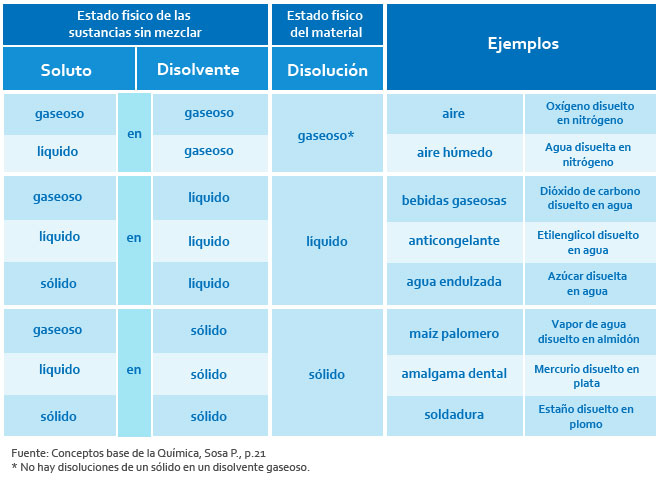
\includegraphics[width = 0.8\textwidth]{dis}
	\caption{Resumen de los distintos tipos de disoluciones}
\end{figure}  

El estudio de las disoluciones en química se hace de vital importancia debido a que la inmensa mayoría de reacciones químicas tienen lugar mediante disoluciones acuosas.

\subsection{Formas de Expresar la Concentración}

Existen varias formas matemáticas de expresar la concentración en una disolución:\\

\begin{definition}[Porcentaje en Masa]
	Se define como la masa de soluto entre la masa total de disolución:
	\begin{align}
		& \%(m/m)=\frac{m_{sol}}{m_{sol}+m_{dvte}}x100
	\end{align}
\end{definition}

\begin{definition}[Porcentaje en Volumen]
Se define como el volumen de soluto entre el volumen total de disolución:
	\begin{align}
	& \%(v/v)=\frac{v_{sol}}{v_{sol}+v_{dvte}}x100
	\end{align}
Se suele utilizar en el caso de disoluciones con solutos líquidos.
\end{definition}

\begin{definition}[Gramos por Litro]
	Se define como los gramos de soluto entre el volumen total en litros de la disolución:
	\begin{align}
		& gr/l =\frac{gr_{sol}}{V(l)_{dison}}
	\end{align}
\end{definition}

\begin{definition}[Molaridad]
	Se define como los moles de soluto entre el volumen total en litros de la disolución:
	\begin{align}
		& M =\frac{n_{sol}}{V(l)_{dison}}
	\end{align}
Es, con diferencia, la más utilizada de todas.
\end{definition}

\begin{definition}[Molalidad]
	Se define como los moles de soluto entre los kilogramos de disolvente:
	\begin{align}
		& m =\frac{n_{sol}}{m(Kgr)_{dvte}}
	\end{align}
\end{definition}

\begin{definition}[Normalidad]
	Se define como los equivalentes de soluto entre el volumen total en litros de la disolución:
	\begin{align}
		& N =\frac{eq_{sol}}{V(l)_{dison}}
	\end{align}
\end{definition}

Debido a su relación con la Molaridad, ambas magnitudes se pueden expresar: \textbf{$N = M\cdot val$}

\begin{definition}[Fracción Molar de Soluto]
Se define como la proporción molar de soluto en la disolución expresada en tanto por uno:
	\begin{align}
		& X_s=\frac{n_{sol}}{n_{sol}+n_{dvte}}
	\end{align}
\end{definition}

\begin{definition}[Fracción Molar de Disolvente]
	Se define como la proporción molar de disolvente en la disolución expresada en tanto por uno:
	\begin{align}
		& X_d=\frac{n_{dvte}}{n_{sol}+n_{dvte}}
	\end{align}
\end{definition}

En ambas fracciones molares se cumple que: \textbf{$X_s + X_d = 1$}\\

En los cálculos con disoluciones se suele utilizar de manera habitual la densidad. Por tanto, es útil recordar que la densidad relaciona la masa de la disolución con el volumen de dicha disolución:\\

\begin{center}
	$d=\frac{m_{dison}}{V_{dison}}$
\end{center}

\begin{exercise}
	\textbf{Un ácido sulfúrico comercial tiene una etiqueta que indica 95 \%(m/m) y  d = 1,83 $gr/cm^3$. Calcula su molaridad, molalidad, normalidad, gramos litro y fracciones molares de soluto y disolvente.}\\
	
	Del dato de porcentaje podemos deducir que en 100 gr de disolución hay 95 gr de soluto puro y por tanto 5 gr de disolvente puro. Por tanto podemos utilizar estos datos para obtener el volumen de la  disolución:\\
	
	$V_{dison}=\frac{M_{dison}}{d}=\frac{100}{1,83}=$ 54,64 ml\\
	
	Por otro lado, y sabiendo que la Masa molecular del ácido sulfúrico es 98 gr/mol, podemos calcular algunas magnitudes:\\
	
	$M = \frac{\frac{95}{98}}{0,05464}=$ 17,74 M\\
	
	$gr/l = \frac{95}{0,05464}=$ 1738,6 gr/l\\
	
	$m = \frac{\frac{95}{98}}{0,005}=$ 19,38 mol/Kg\\
	
	Puesto que el $H_2SO_4$ contiene dos hidrógenos, su valencia es dos y, por tanto, su Normalidad:\\
	
	$N=M\cdot val=17,74\cdot 2=$ 35,48 N\\
	
	Y sus fracciones molares de soluto y disolvente:\\
	
	$X_s = \frac{\frac{95}{98}}{\frac{95}{98}+\frac{5}{18}}= 0,78$\\
	
	$X_d=1-X_s=0,22$
\end{exercise}

\subsection{Diluciones}

Se puede definir una dilución en una disolución acuosa como el proceso de añadir agua pura a una alícuota de una disolución concentrada para que su concentración sea menor. En un laboratorio químico es una tarea bastante común puesto que muchos compuestos que se utilizan de manera muy habitual (cómo algunos ácidos inorgánicos) suelen venir en forma de disolución muy concentrada. El cálculo de diluciones se basa en el hecho de que el número de moles de soluto presentes en la alícuota de la disolución concentrada es el mismo que en la disolución diluida, pues la variación de la concentración de la disolución se debe al aumento del volumen de la misma.\\

\begin{center}
	$n_{conc}=n_{dil}$
\end{center}

Y sustituyendo en la definición de Molaridad:\\

\begin{center}
	$V_{conc}\cdot M_{conc}=V_{dil}\cdot M_{dil}$
\end{center}

\begin{exercise}
	\textbf{Queremos preparar 250 ml de una disolución 0,5 M de Ácido Sulfúrico a partir de una disolución comercial de 95 \% (m/m) y d = 1,83 $gr/cm^3$. Calcula el volumen necesario que debemos tomar de la disolución comercial para obtener la dilución.}\\
	
	Lo primero que debemos de hacer es expresar la concentración del ácido comercial en molaridad (pues lo más común es que las etiquetas nos indiquen densidad y porcentaje en masa). Omitiremos los cálculos, puesto que son los mismos que en el ejercicio anterior. Por tanto, una disolución 95 \%(m/m) y de densidad 1,83 $gr/cm^3$ es equivalente a una disolución 17,74 M. Por ello, y teniendo en cuenta que el número de moles de soluto no varía en la disolución comercial:\\
	
	$V_{conc}\cdot M_{conc}=V_{dil}\cdot M_{dil}$\\
	
	Como nos piden el volumen de la concentrada:\\
	
	$V_{conc}=\frac{V_{dil}\cdot M_{dil}}{M_{conc}}= \frac{250\cdot 0,5}{17,74}=$ 7 ml\\
		
	Luego si cogemos una alícuota de 7 ml de la disolución comercial y completamos en un matraz aforado hasta los 250 ml, obtendremos una disolución 0,5 M.
	
\end{exercise}

\section{Estequiometría}

Se puede definir Estequiometría como el cálculo de las relaciones cuantitativas entre los reactivos y los productos de una reacción química. Estas relaciones se pueden deducir en base a la teoría atómica, aunque históricamente se desarrollaron siguiendo principios y leyes empíricas.Constituye en si misma uno de los pilares básicos del trabajo en el laboratorio, por lo que se hace imprescindible su estudio en esta asignatura.

\subsection{Ajuste de Reacciones Químicas}

Una reacción química se puede definir como un cambio en la ordenación de los átomos entre los reactivos y los productos para dar compuestos químicos totalmente distinto. Puesto que ningún proceso químico puede violar la Ley de Lavoisier de Conservación de la Masa, se hace necesario antes de entrar en cualquier consideración de carácter cuantitativo asegurarse que el numero total de átomos presentes tanto en reactivos como en productos sean iguales (ya que la materia se conserva y ningún átomo puede aparecer o desaparecer de la nada) A este proceso se le conoce como \textbf{Ajuste de una Reacción Química}.\\

Por ejemplo, para la reacción de formación del agua:\\

\begin{center}
	$H_2 + O_2 \longrightarrow H_2O$
\end{center}

Si observamos bien nos daremos cuenta que en el balance global de átomos, a la derecha solo hay un átomo de oxígeno y a la derecha dos. La forma de solventar esto sería multiplicar por dos el agua. Pero si multiplicamos el agua se nos modifica tanto el número de oxígenos como el número de hidrógenos, por lo que habría que multiplicar por dos también el hidrógeno molecular, quedándose totalmente ajustada la reacción.\\

\begin{center}
	$2H_2 + O_2 \longrightarrow 2H_2O$
\end{center}

Por lo tanto para que se cumpla la Ley de Conservación de la Masa tiene que ocurrir que:\\

\begin{center}
\textbf{2 moléculas de Hidrógeno reaccionan con una molécula de Oxígeno para dar 2 moléculas de agua}
\end{center}

La escala atómica es demasiado pequeña para manipularse en un laboratorio. Pero como la reacción es proporcional también se puede cumplir tomando como referencia el mol. Así pues:\\

\begin{center}
\textbf{2 moles de Hidrógeno reaccionan con un mol de Oxígeno para dar 2 moles de agua}
\end{center}

\subsection{Estequimetría con un Reactivo en Exceso}

Sería el caso mas simple de todos, aquel en el que la cantidad de un reactivo es lo suficientemente mayor como para que no haya que tenerlo en cuenta a la hora de hacer los cálculos.\\

\begin{exercise}
	\textbf{Se hacen reaccionar 15 gr de Hidrógeno con exceso de oxígeno. Calcula la cantidad de agua formada.}\\
	
	Escribimos la reacción química:\\
	
	\begin{center}
		$2H_2 + O_2 \longrightarrow 2H_2O$
	\end{center}
	
	Calculamos después los moles de hidrógeno que se hacen reaccionar:\\
	
	n = 15 / 2 = 7,5 moles de Hidrógeno\\
	
	Y ahora planteamos un regla de tres con la proporción que nos indica la reacción:\\
	\begin{equation*}
	
	2 moles de $H_2$ \hline 1 mol $O_2$\\
	
	7,5 moles de $H_2$ \hline x mol $O_2$
	\right |
	\quad\text{x = 3,75 moles de $O_2$}
	\end{equation*}
\end{exercise}